\documentclass[12pt]{article}

\usepackage{../gongkechuang}

\title{EI313-Hugepage Benchmark}

\begin{document}

\maketitle

In this report, the performance of virtual machines running with different huge page settings, i.e. No huge pages, transparent huge pages, and traditional static-appointed huge pages in 2MB and 1GB, are compared.

\section{Introduction}

Page tables are key to multi-processing and are one of the fundamental parts of a modern time-sharing operating system. Memory is organized into pages, while page entries are stored in the translation look-aside buffer (TLB), which is critical for fast memory addressing. Larger page sizes can reduce the page entries, and finally reduce the TLB miss and reach higher efficiency.

On the x86\_64 architecture, the default page size is 4KB, while huge tables are supported in a selection of CPU, namely pse for 2MB pages, and pdpe1gb for 1GB pages.

Linux has already introduced the transparent huge page mechanism, which is organized by the kernel to merge normal pages into default 2MB pages to increase efficiency. Traditional huge page management methods can also be taken. 1GB pages cannot be utilized with transparent huge page mechanism, as Linux kenel doesn’t implement them, and not much programs can utilize more than 1GB memory.

QEMU/KVM, by default, will not use the dedicated huge page. This means that the normal pages, or transparent huge pages organized by the system, will be used. Dedicated huge pages may be allocated either statically at boot time with boot parameters or dynamically at runtime. However, dynamical huge pages are more complicated to allocate, as other programs will start to occupy the memory and a clean and continuous block will be difficult to allocate if not at system boot time, which is especially difficult with 1GB pages.

In this report, we compared the efficiency of transparent huge pages, dedicated huge pages in 1GB and 2MB, and without huge pages.

\section{Environmental Configuration}

The script we are describing below, \texttt{hugepage.sh}, can be downloaded from GitHub at \textcolor{blue}{\href{https://gist.github.com/Victrid/bcd412e0f7e421ec6b4b2fffc3da4923}{here}}.

\subsection{Host Configuration}

Huge page configurations are set at boot time with Linux kernel parameters. This can be done by modifying \texttt{\$\{GRUB\_CMDLINE\_LINUX\}} value in \texttt{/etc/default/grub}, but this needs to be adjusted every time. In our testing environment, we adjusted \texttt{/etc/grub.d/10\_linux}, by adding different boot options to the grub.

Our current system boots into the graphic mode (level 5), where multiple applications will affect the result. Huge pages only provide a slight efficiency boost, and this disturbing can cause wrong results in comparing. To minimize the effect, we also boot the system into the multiuser mode with networking (level 3). The core part is to add the \texttt{hugepagesz}, \texttt{hugepages} and \texttt{transparent\_hugepage} boot options.

\lstinputlisting[
	language=bash,
	linerange={81-100},
	firstnumber=81,
	breaklines=true,
	postbreak=\mbox{\textcolor{red}{$\hookrightarrow$}}, prebreak=\mbox{\textcolor{red}{$\swarrow$}},
	caption={Boot parameter modification}
]{hugepage.sh}
\lstinputlisting[
	language=bash,
	linerange={ 104-108},
	firstnumber=104,
	breaklines=true,
	postbreak=\mbox{\textcolor{red}{$\hookrightarrow$}}, prebreak=\mbox{\textcolor{red}{$\swarrow$}},
	nolol
]{hugepage.sh}

\begin{figure}[h]
	\centering
	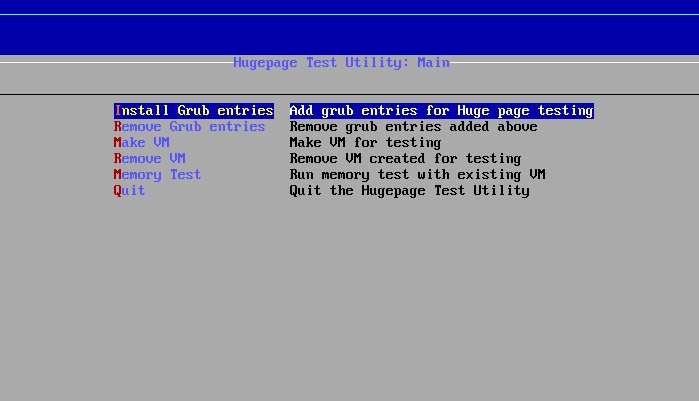
\includegraphics[width=0.8\textwidth]{fig1.png}
	\caption{Hugepage Test Utility}
	\label{fig:hpt}
\end{figure}

As in figure \ref{fig:hpt}, the \textbf{Install} option will detect the \texttt{pse} and \texttt{pdpe1gb} flags, and install the grub entries respectively. It will also install the with or without transparent pages options to the grub menu. The \textbf{Remove} option can remove the grub entries installed without touching \texttt{/etc/default/grub}, which will be a safer option than modifying \texttt{/etc/default/grub} itself.

The huge page information from \texttt{/proc/meminfo} are shown in the figure \ref{fig:mem}. \texttt{AnonHugePages} shows current transparent hugepage usage, and \texttt{Hugepagesize} shows the huge page size, while the \texttt{Hugetlb} shows the current dedicated huge page table total size.

\begin{figure}[h]
	\centering
	\hfill
	\begin{subfigure}[b]{0.4\textwidth}
		\centering
		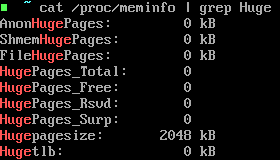
\includegraphics[width=\textwidth]{fig7-4.png}
		\caption{No Huge Page}
	\end{subfigure}
	\hfill
	\begin{subfigure}[b]{0.4\textwidth}
		\centering
		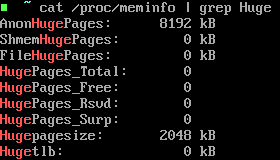
\includegraphics[width=\textwidth]{fig7-3.png}
		\caption{Transparent Huge Page}
	\end{subfigure}
	\hfill

	\hfill
	\begin{subfigure}[b]{0.4\textwidth}
		\centering
		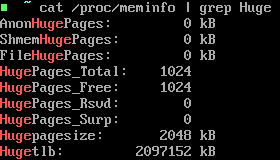
\includegraphics[width=\textwidth]{fig7-1.png}
		\caption{2KB Huge page}
	\end{subfigure}
	\hfill
	\begin{subfigure}[b]{0.4\textwidth}
		\centering
		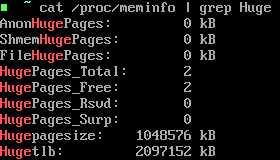
\includegraphics[width=\textwidth]{fig7-2.png}
		\caption{1GB Huge page}
	\end{subfigure}
	\hfill
	\caption{\texttt{/proc/meminfo} Information}
	\label{fig:mem}
\end{figure}

A memory usage example when a VM using 2MB huge pages is shown in figure \ref{fig:running}. We can see that \texttt{HugePages\_Free} decreased from 1024 to 0.

\begin{figure}[h]
	\centering
	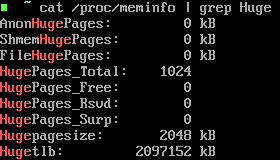
\includegraphics[width=0.4\textwidth]{fig8.png}
	\caption{VM with 2MB Huge Pages Running}
	\label{fig:running}
\end{figure}

\subsection{Virtual Machine Configuration}

The VM can be configured to use the huge pages by adding these XML in the virt-manager definition script.

\begin{lstlisting}[language=xml]
<memoryBacking>
  <hugepages/>
</memoryBacking>
\end{lstlisting}

However, when the transparent huge pages or no huge pages are configured, VM defined with this can fail to start. The \textbf{Make VM} option can build the testing virtual machines with our XML definition files and VM disk images provided by Arch Linux and \texttt{mirror.sjtu.edu.cn}, with or without huge pages. The \textbf{Memory Test} option will detect which huge page configuration the system is currently running with by checking \texttt{/proc/meminfo}, and run the benchmark with a correct VM. After testing, \textbf{Remove VM} option can remove the VM registered with this script.

\begin{figure}[h]
	\centering
	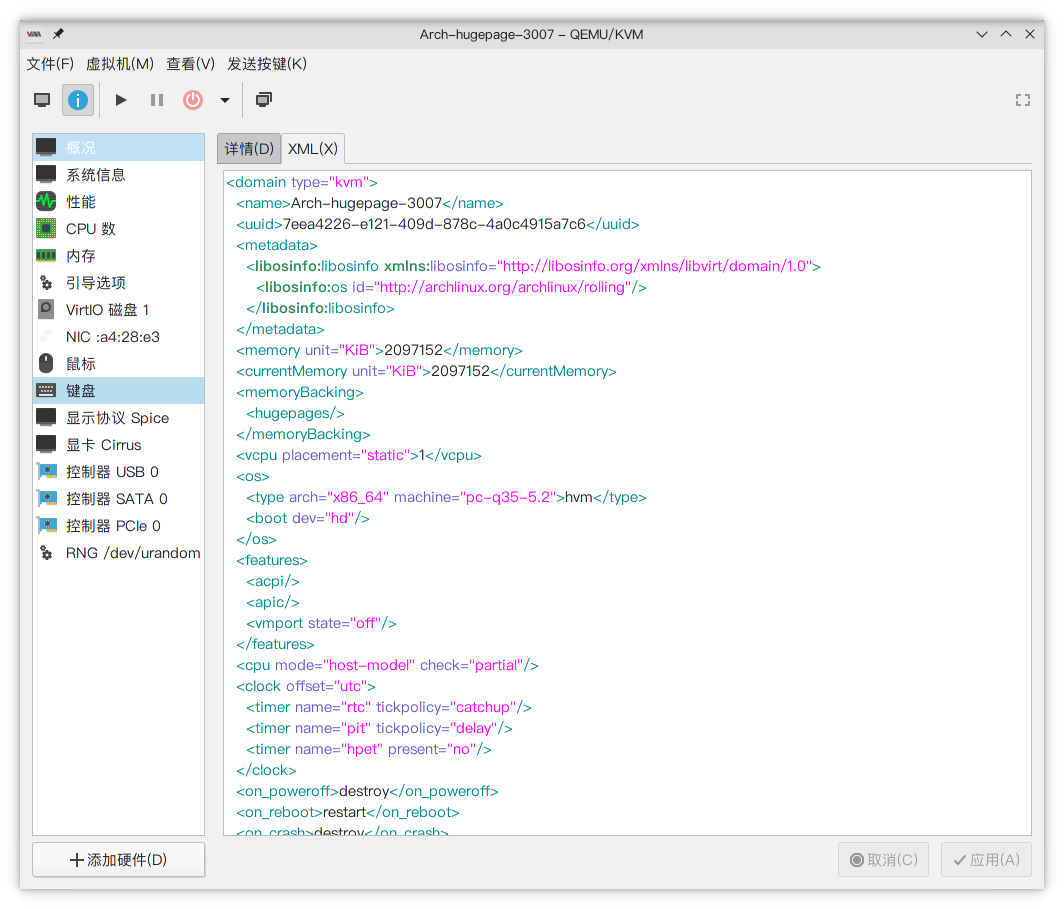
\includegraphics[width=0.7\textwidth]{fig2.png}
	\caption{One of defined VM with hugepages}
	\label{fig:df}
\end{figure}

\lstinputlisting[
	language=bash,
	linerange={473-482},
	firstnumber=473,
	breaklines=true,
	postbreak=\mbox{\textcolor{red}{$\hookrightarrow$}}, prebreak=\mbox{\textcolor{red}{$\swarrow$}},
	caption={Hugepage environment check}
]{hugepage.sh}

\lstinputlisting[
	language=bash,
	linerange={629-640},
	firstnumber=629,
	breaklines=true,
	postbreak=\mbox{\textcolor{red}{$\hookrightarrow$}}, prebreak=\mbox{\textcolor{red}{$\swarrow$}},
	nolol
]{hugepage.sh}

\subsection{Virtualization host}

The virtualization host that I used for my experiments has 16GB of RAM with a 2-core (4 thread) Intel i7-5500U. This processor has a maximum clock speed of 3.0GHz. Total L1, L2, and L3 cache sizes are 32KB, 256KB, and 4MB, respectively. The memory is 8GBx2 DDR3, from different manufacturers, but the spec are the same. Table \ref{tbl:hst} summarizes the specifications for the host.

\begin{table}[h]
	\centering \scriptsize \ttfamily {
		\begin{tabular}{c|l}
			\hline
			Processor            & Intel i7-5500U                          \\ \hline
			Memory size          & 15880MB                                 \\ \hline
			Memory details       & 8GB SODIMM DDR3 by Kingston and Samsung \\ \hline
			Device               & 20BVA03NCD ThinkPad T450                \\ \hline
			OS                   & Arch Linux                              \\ \hline
			Linux kernel version & \texttt{5.15.7-arch1-1}                 \\ \hline
			QEMU version         & \texttt{5.2.0-4}                        \\ \hline
		\end{tabular}
	}
	\caption{Host Specs} \label{tbl:hst}
\end{table}

\subsection{Virtual machines}

The virtual machines are defined in XML embedded in the script. The script will download the VM disk images, which has Arch Linux pre-installed. All virtual machines with or without huge pages are configured with 1 CPU and 2GB memory. A part of the VM specification are shown in the figure \ref{fig:df}.

\section{Benchmarking}

\textbf{Sysbench} is a modular, cross-platform and multi-threaded benchmark tool for evaluating OS parameters that are important for a system running a database under intensive load. For database testing, it can test both MySQL and PostgreSQL. We uses sysbench to test the memory sequential and random read and write. The sysbench also allows testing with hugepages inside the VM.

The sysbench we used for testing was version \texttt{1.0.20-1} from Arch official community repository. The installation is performed with Arch Linux’s standard packaging utility \texttt{pacman}.

\lstinputlisting[
	language=bash,
	linerange={548-563},
	firstnumber=548,
	breaklines=true,
	postbreak=\mbox{\textcolor{red}{$\hookrightarrow$}}, prebreak=\mbox{\textcolor{red}{$\swarrow$}},
	caption={Installing Sysbench on VM}
]{hugepage.sh}

The memory testing can be changed with \texttt{--memory-hugetlb[=on|off]} options on the VM. We tested that the QEMU does not support 1GB hugepages inside the VM, so only THP, no HP and 2MB HP are tested.

As we mentioned above, the memory is a constantly changing part, and all processes running inside or outside the VM will disturb them. We let the benchmark run for 500 times, to minimize the effect of memory fluctuations.

\lstinputlisting[
	language=bash,
	linerange={618-625},
	firstnumber=618,
	breaklines=true,
	postbreak=\mbox{\textcolor{red}{$\hookrightarrow$}}, prebreak=\mbox{\textcolor{red}{$\swarrow$}},
	caption={Sysbench benchmark}
]{hugepage.sh}

The raw result is shown in table \ref{tbl:raw}. The huge page result is shown in table \ref{tbl:ins}.

\begin{table}[]
	{\scriptsize \ttfamily
		\begin{tabular}{c|c|c|c|c}
			\hline
			                                                               & \begin{tabular}[c]{@{}c@{}}Sequential \\ R/W\end{tabular}            & \begin{tabular}[c]{@{}c@{}}Random \\ R/W\end{tabular}             & \begin{tabular}[c]{@{}c@{}}Sequential\\ Latency\end{tabular}                        & \begin{tabular}[c]{@{}c@{}}Random\\ Latency\end{tabular}                                \\ \hline
			No Hugepage                                                    & \begin{tabular}[c]{@{}c@{}}12385.43 MB/s\\ 9173.66 MB/s\end{tabular} & \begin{tabular}[c]{@{}c@{}}363.98 MB/s\\ 363.99 MB/s\end{tabular} & \begin{tabular}[c]{@{}c@{}}Max: 28.77ms/30.30ms\\ Avg: 5.165ms/6.975ms\end{tabular} & \begin{tabular}[c]{@{}c@{}}Max: 185.97ms/181.42ms\\ Avg: 175.83ms/175.82ms\end{tabular} \\ \hline
			\begin{tabular}[c]{@{}c@{}}Transparent\\ Hugepage\end{tabular} & \begin{tabular}[c]{@{}c@{}}12675.91 MB/s\\ 9191.84 MB/s\end{tabular} & \begin{tabular}[c]{@{}c@{}}404.90 MB/s\\ 369.92 MB/s\end{tabular} & \begin{tabular}[c]{@{}c@{}}Max: 35.77ms/33.70ms\\ Avg: 5.047ms/6.961ms\end{tabular} & \begin{tabular}[c]{@{}c@{}}Max: 167.27ms/181.62ms\\ Avg: 158.06ms/173.01ms\end{tabular} \\ \hline
			\begin{tabular}[c]{@{}c@{}}2MB\\ Hugepage\end{tabular}         & \begin{tabular}[c]{@{}c@{}}12669.97 MB/s\\ 9196.24 MB/s\end{tabular} & \begin{tabular}[c]{@{}c@{}}405.21 MB/s\\ 369.59 MB/s\end{tabular} & \begin{tabular}[c]{@{}c@{}}Max: 29.06ms/33.97ms\\ Avg: 5.050ms/6.958ms\end{tabular} & \begin{tabular}[c]{@{}c@{}}Max: 167.53ms/182.70ms\\ Avg: 157.18ms/172.72ms\end{tabular} \\ \hline
			\begin{tabular}[c]{@{}c@{}}1GB\\ Hugepage\end{tabular}         & \begin{tabular}[c]{@{}c@{}}12643.97 MB/s\\ 9314.89 MB/s\end{tabular} & \begin{tabular}[c]{@{}c@{}}407.17 MB/s\\ 370.54 MB/s\end{tabular} & \begin{tabular}[c]{@{}c@{}}Max: 31.93ms/32.88ms\\ Avg: 5.060ms/6.869ms\end{tabular} & \begin{tabular}[c]{@{}c@{}}Max: 166.63ms/182.91ms\\ Avg: 157.94ms/173.16ms\end{tabular} \\ \hline
		\end{tabular}}
	\caption{Raw result of memory benchmark} \label{tbl:raw}
\end{table}

\begin{table}[]
	\centering
	{\scriptsize \ttfamily
		\begin{tabular}{c|c|c|c}
			\hline
			Host\textbackslash VM                                   & No HP                                                             & \begin{tabular}[c]{@{}c@{}}Transparent\\ HP\end{tabular}          & 2M HP                                                            \\ \hline
			\begin{tabular}[c]{@{}c@{}}2MB \\ Hugepage\end{tabular} & \begin{tabular}[c]{@{}c@{}}352.05 MB/s\\ 339.45 MB/s\end{tabular} & \begin{tabular}[c]{@{}c@{}}405.21 MB/s\\ 369.59 MB/s\end{tabular} & \begin{tabular}[c]{@{}c@{}}439.57MB/s\\ 379.49MB/s\end{tabular}  \\ \hline
			\begin{tabular}[c]{@{}c@{}}1GB\\ Hugepage\end{tabular}  & \begin{tabular}[c]{@{}c@{}}372.96 MB/s\\ 347.39 MB/s\end{tabular} & \begin{tabular}[c]{@{}c@{}}407.17 MB/s\\ 370.54 MB/s\end{tabular} & \begin{tabular}[c]{@{}c@{}}463.08 MB/s\\ 368.48MB/s\end{tabular} \\ \hline
		\end{tabular}
	}
	\caption{Huge page inside VM} \label{tbl:ins}
\end{table}

\section{Analysis}

\paragraph{Sequential R/W} Sequential read and write speed are shown in the figure \ref{fig:seq}.

\begin{figure}[h]
	\centering
	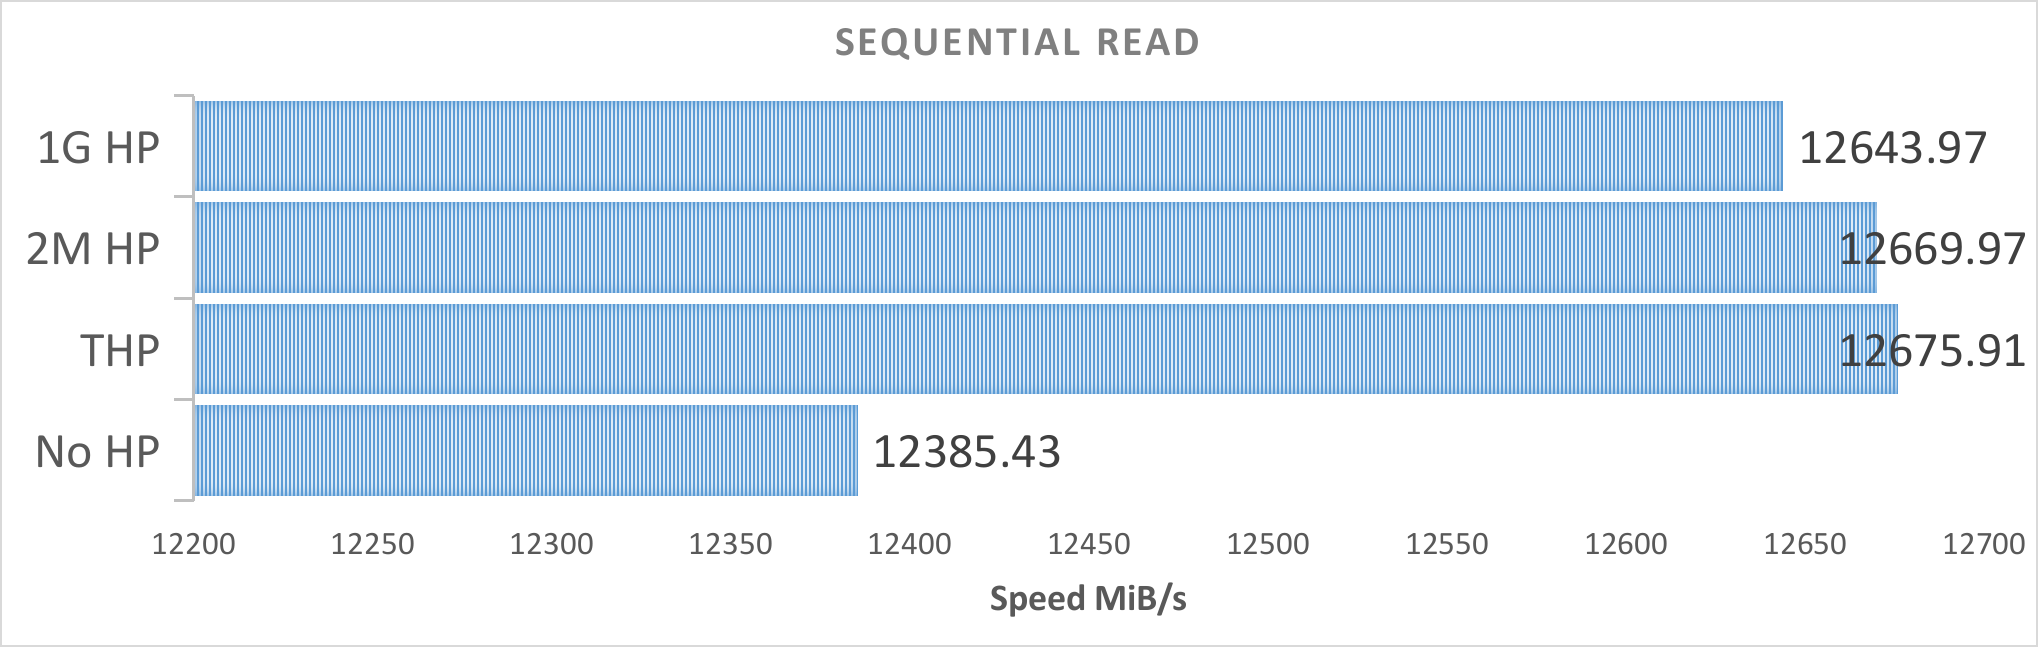
\includegraphics[width=0.8\textwidth]{fig3.png}

	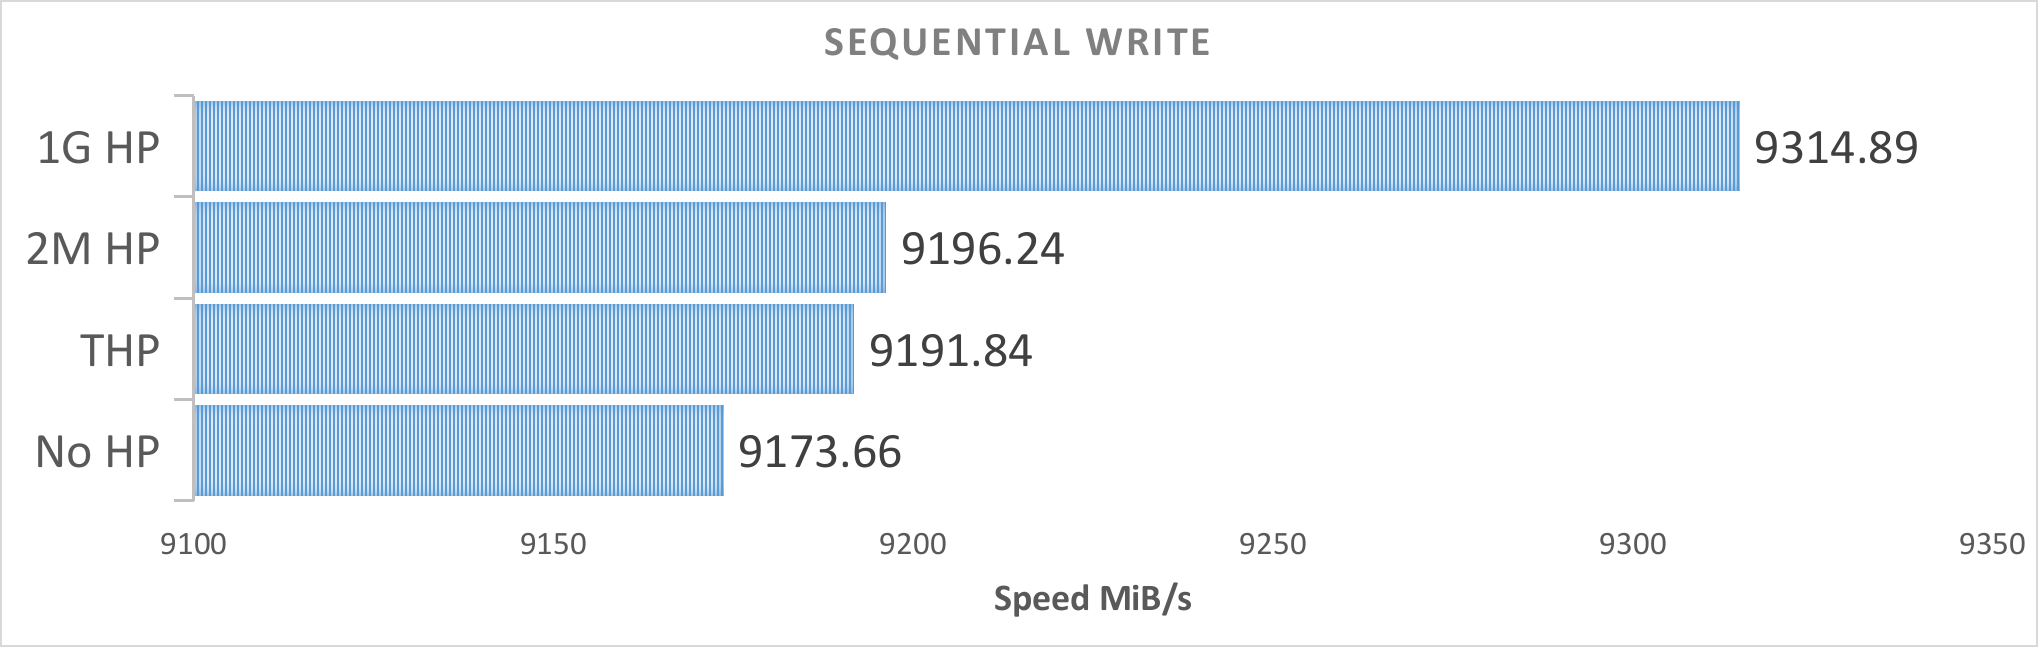
\includegraphics[width=0.8\textwidth]{fig4.png}
	\caption{Sequential Read and Write}
	\label{fig:seq}
\end{figure}

It shows that in sequential read, using huge page can lead up to \textbf{2.3\% efficiency increase}, but the speed variance between different huge page implementation are not significant. However, in sequential write, the 1G huge page gains up to \textbf{1.5\% efficiency increase} than smaller 2M huge pages and no huge page (i.e. 4KB page size).

\paragraph{Random R/W} Random read and write speed are shown in the figure \ref{fig:rdm}.

\begin{figure}[h]
	\centering
	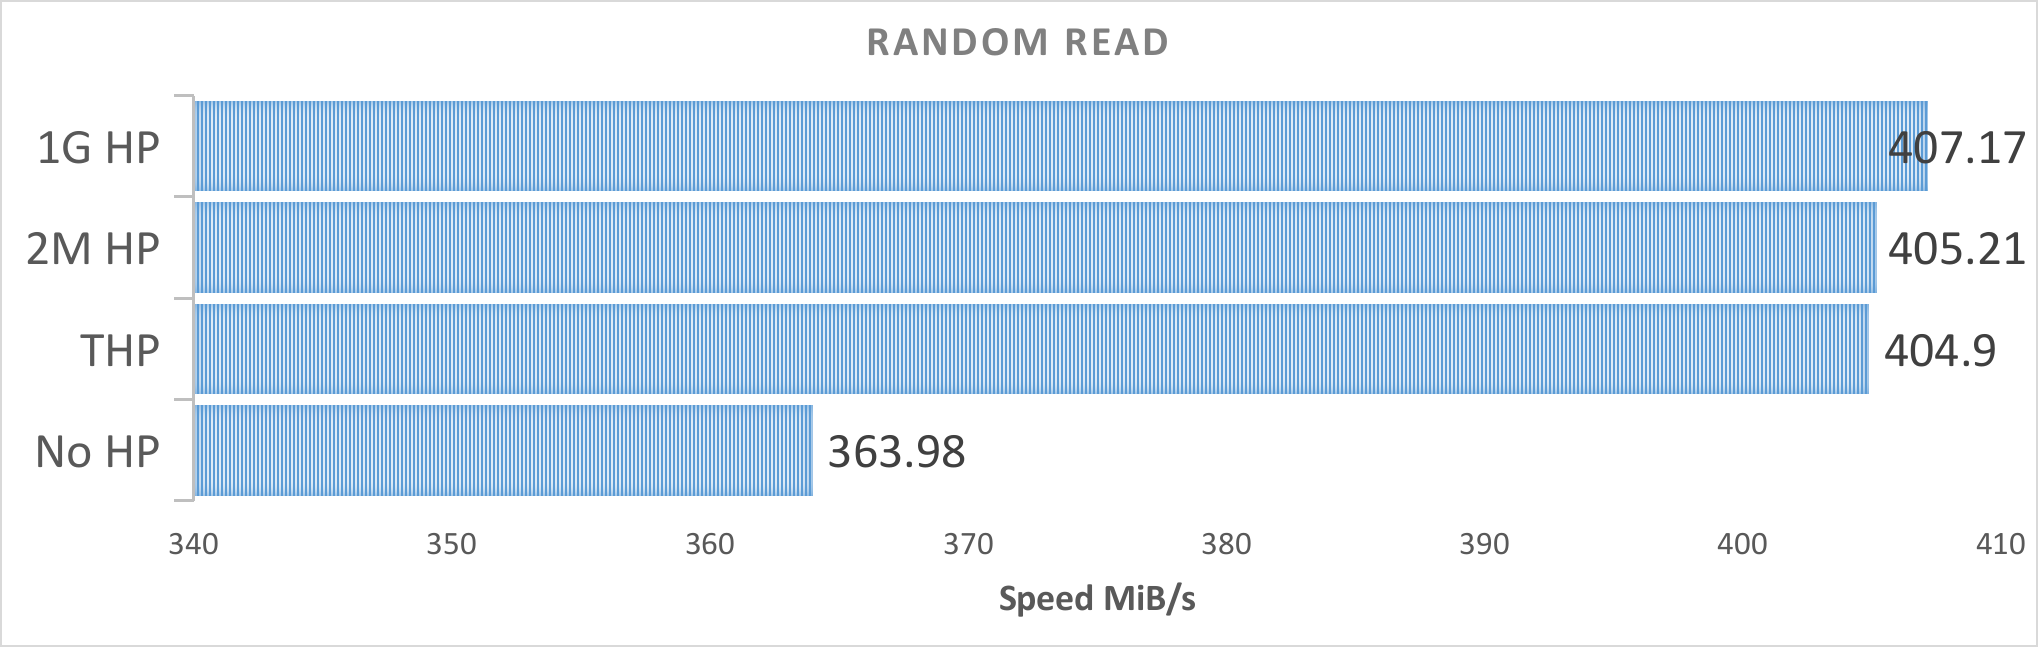
\includegraphics[width=0.8\textwidth]{fig5.png}

	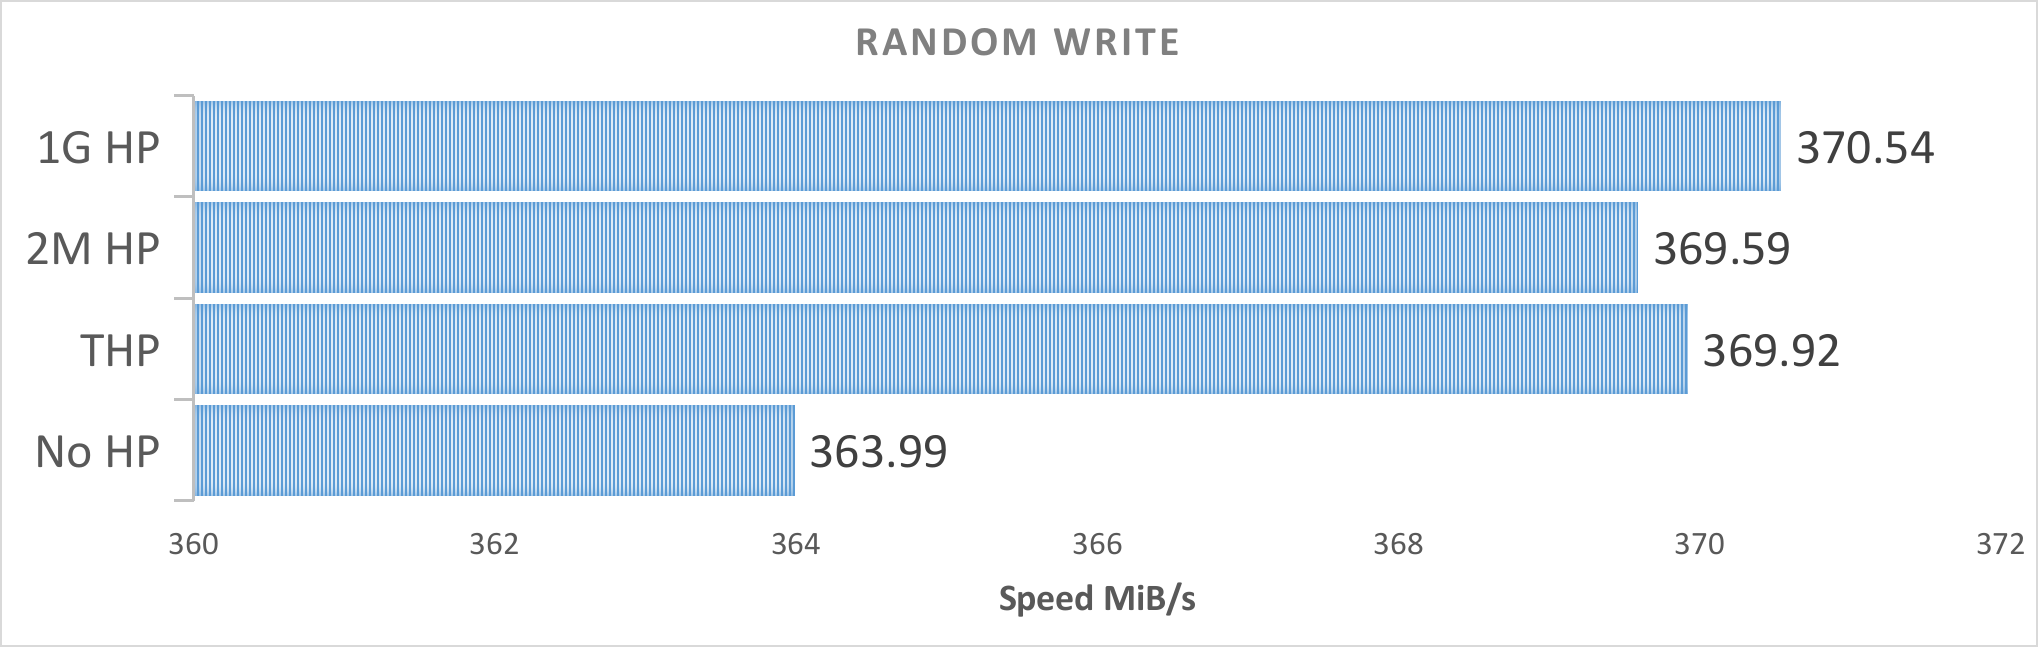
\includegraphics[width=0.8\textwidth]{fig6.png}
	\caption{Random Read and Write}
	\label{fig:rdm}
\end{figure}

It shows that in random read, using huge page can lead up to 11.8\% efficiency increase, and in random write this is 1.7\%. In both random read and write, the 1G huge page has the best performance.

This is because that huge pages can reduce the TLB miss when CPU is translating the actual memory address, and larger huge pages can leads to better result. For these results, It should be noticed that this generation (haswell) has different sizes of TLBs for diffrent size of pages, namely 4 entries for 1GB pages, 32 entries for 2MB pages, and 64 entries for 4KB pages, separately. This leads to different result in sequential reading.

\paragraph{Transparent Huge page, and nested huge page} Using huge pages can lead to better performance than no huge pages, both on the host and VM. It should also be noticed that the transparent huge page has nearly the same performance with the dedicated 2M huge page on host, but inside the VM the dedicated huge page seems to have better result than transparent huge page. We doubt that this is due to sysbench's misleading design. In the \texttt{--memory-hugetlb=on} option, the sysbench will acquire the memory from the hugeTLB API, but a maximum of 1 page is utilized during the test, making it a trick to increase the actual speed by accessing the same page over and over. This increased the reading speed by a lot. We think this result has not much significance, so we didn't make the quantitative comparison.

\paragraph{Conclusion} The benchmark shows that the best performance comes with 1GB dedicated hugepage, and no matter which huge page implementation can increase the memory efficiency. To our surprise, the transparent huge page has nearly the same performance with the dedicated 2M huge page, while transparent huge page does not need much configuration, and the memory can be utilized more efficiently, as only a small amount of programs like postgresql and QEMU/KVM can utilize them. These dedicated huge pages in 1GB can only be effectively used having the programs mentioned above constantly running, like a SQL server or virtualization center. For normal computers with most of applications unable to use these huge pages, it is probably better to use the transparent huge page mechanism instead.

\section{Conclusion}
\emph{omitted}
\end{document}
